% answers.tex —— 2002 年·春季京蒙皖卷·文科 · 参考答案与详细解析片段
% 由 tools/generate_projects.py 依来源总账自 2002/2002_数学真题_春季京蒙皖文_试题.md + 2002/2002_数学真题_春季京蒙皖文_解析正文.md + 2002/2002_数学真题_春季京蒙皖文_答案要点.md 生成，勿手改（改源 MD 后重跑）


\begin{gktip}
固定源 PDF 为印刷页码 97–98 的两页题面，不附答案。以下解析均依据题面独立复算；第 15、19 题图形在 LaTeX 工程中以 TikZ/PGFPlots 矢量源重绘。
\end{gktip}

\gkpart{一、选择题}

\begin{answer}
\gksolhead{1}{}

\textbf{题目}：

\Needspace{5\baselineskip}
不等式组

\nopagebreak[4]
\[
\begin{cases}
x^2-1<0,\\
x^2-3x<0
\end{cases}
\]

的解集为\mbox{（　　）}

（A）$\{x\mid -1<x<1\}$　　（B）$\{x\mid 0<x<3\}$

（C）$\{x\mid 0<x<1\}$　　（D）$\{x\mid -1<x<3\}$

\Needspace{4\baselineskip}
\textbf{解析}

由 $x^2-1<0$ 得 $-1<x<1$，由 $x^2-3x<0$ 得 $0<x<3$，两者交集为 $(0,1)$，选 C。

\gkanswer{答案：C。}

\end{answer}
\begin{answer}
\gksolhead{2}{}

\textbf{题目}：

已知三条直线 $m\text{、}n\text{、}l$，三个平面 $\alpha\text{、}\beta\text{、}\gamma$，下列四个命题中，正确的是\mbox{（　　）}

（A）$\begin{cases}\alpha\perp\gamma,\\ \beta\perp\gamma\end{cases}\Rightarrow\alpha\parallel\beta$

（B）$\begin{cases}m\parallel\beta,\\ l\perp m\end{cases}\Rightarrow l\perp\beta$

（C）$\begin{cases}m\parallel\gamma,\\ n\parallel\gamma\end{cases}\Rightarrow m\parallel n$

（D）$\begin{cases}m\perp\gamma,\\ n\perp\gamma\end{cases}\Rightarrow m\parallel n$

\Needspace{4\baselineskip}
\textbf{解析}

两个都垂直于同一平面的直线彼此平行，因此 D 正确。其余命题缺少必要的相交或垂直条件。

\gkanswer{答案：D。}

\end{answer}
\begin{answer}
\gksolhead{3}{}

\textbf{题目}：

已知椭圆的焦点是 $F_1\text{、}F_2$，$P$ 是椭圆上的一个动点。如果延长 $F_1P$ 到 $Q$，使得 $|PQ|=|PF_2|$，那么动点 $Q$ 的轨迹是\mbox{（　　）}

（A）圆　　（B）椭圆　　（C）双曲线的一支　　（D）抛物线

\Needspace{4\baselineskip}
\textbf{解析}

\Needspace{5\baselineskip}
由 $Q$ 在 $F_1P$ 的延长线上且 $PQ=PF_2$，得

\nopagebreak[4]
\[
F_1Q=F_1P+PQ=F_1P+PF_2=2a.
\]

所以 $Q$ 到定点 $F_1$ 的距离恒定，轨迹为圆，选 A。

\gkanswer{答案：A。}

\end{answer}
\begin{answer}
\gksolhead{4}{}

\textbf{题目}：

\Needspace{5\baselineskip}
如果 $\theta\in\left(\dfrac\pi2,\pi\right)$，那么复数

\nopagebreak[4]
\[
(1+i)(\cos\theta+i\sin\theta)
\]

的辐角的主值是\mbox{（　　）}

（A）$\theta+\dfrac{9\pi}{4}$　　（B）$\theta+\dfrac\pi4$　　（C）$\theta-\dfrac\pi4$　　（D）$\theta+\dfrac{7\pi}{4}$

\Needspace{4\baselineskip}
\textbf{解析}

复数 $(1+i)(\cos\theta+i\sin\theta)$ 的辐角为 $\theta+\pi/4$。由于 $\theta\in(\pi/2,\pi)$，该值在 $(3\pi/4,5\pi/4)$ 内，已经是主值范围内的值，选 B。

\gkanswer{答案：B。}

\end{answer}
\begin{answer}
\gksolhead{5}{}

\textbf{题目}：

若角 $\alpha$ 满足 $\sin2\alpha<0$，$\cos\alpha-\sin\alpha<0$，则 $\alpha$ 在\mbox{（　　）}

（A）第一象限　　（B）第二象限　　（C）第三象限　　（D）第四象限

\Needspace{4\baselineskip}
\textbf{解析}

$\sin2\alpha<0$ 时 $\alpha$ 在第二或第四象限。第二象限中 $\cos\alpha<0<\sin\alpha$，满足 $\cos\alpha-\sin\alpha<0$；第四象限中 $\cos\alpha>0>\sin\alpha$，不满足。故选 B。

\gkanswer{答案：B。}

\end{answer}
\begin{answer}
\gksolhead{6}{}

\textbf{题目}：

从 6 名志愿者中选出 4 人分别从事翻译、导游、导购、保洁四项不同工作。若其中甲、乙两名志愿者都不能从事翻译工作，则选派方案共有\mbox{（　　）}

（A）280 种　　（B）240 种　　（C）180 种　　（D）96 种

\Needspace{4\baselineskip}
\textbf{解析}

\Needspace{5\baselineskip}
翻译工作只能从其余 4 人中选 1 人，有 $4$ 种；其余 3 项从剩下 5 人中排列，有 $P_5^3$ 种。因此

\nopagebreak[4]
\[
4P_5^3=4\cdot5\cdot4\cdot3=240,
\]

选 B。

\gkanswer{答案：B。}

\end{answer}
\begin{answer}
\gksolhead{7}{}

\textbf{题目}：

在 $\triangle ABC$ 中，$AB=2$，$BC=1.5$，$\angle ABC=120^\circ$。若使三角形绕直线 $BC$ 旋转一周，则所形成的几何体的体积是\mbox{（　　）}

（A）$\dfrac32\pi$　　（B）$\dfrac52\pi$　　（C）$\dfrac72\pi$　　（D）$\dfrac92\pi$

\Needspace{4\baselineskip}
\textbf{解析}

\Needspace{5\baselineskip}
点 $A$ 到直线 $BC$ 的距离为 $AB\sin120^\circ=\sqrt3$。绕 $BC$ 旋转所得为底面半径 $\sqrt3$、高 $BC=1.5$ 的圆锥，故

\nopagebreak[4]
\[
V=\frac13\pi(\sqrt3)^2\cdot1.5=\frac32\pi.
\]

选 A。

\gkanswer{答案：A。}

\end{answer}
\begin{answer}
\gksolhead{8}{}

\textbf{题目}：

到两坐标轴距离相等的点的轨迹方程是\mbox{（　　）}

（A）$x-y=0$　　（B）$x+y=0$　　（C）$|x|-y=0$　　（D）$|x|-|y|=0$

\Needspace{4\baselineskip}
\textbf{解析}

点到两坐标轴的距离分别为 $|y|$、$|x|$，距离相等即 $|x|=|y|$，选 D。

\gkanswer{答案：D。}

\end{answer}
\begin{answer}
\gksolhead{9}{}

\textbf{题目}：

函数 $y=2\sin x$ 的单调区间是\mbox{（　　）}

（A）$\left[2k\pi-\dfrac\pi2,2k\pi+\dfrac\pi2\right]$（$k\in\mathbb Z$）

（B）$\left[2k\pi+\dfrac\pi2,2k\pi+\dfrac{3\pi}2\right]$（$k\in\mathbb Z$）

（C）$[2k\pi-\pi,2k\pi]$（$k\in\mathbb Z$）

（D）$[2k\pi,2k\pi+\pi]$（$k\in\mathbb Z$）

\Needspace{4\baselineskip}
\textbf{解析}

$y=2\sin x$ 在每个区间 $\left[2k\pi-\pi/2,2k\pi+\pi/2\right]$ 上递增，选 A。

\gkanswer{答案：A。}

\end{answer}
\begin{answer}
\gksolhead{10}{}

\textbf{题目}：

\Needspace{5\baselineskip}
在

\nopagebreak[4]
\[
\left(\frac1x+x^2\right)^6
\]

的展开式中，$x^3$ 的系数和常数项依次是\mbox{（　　）}

（A）20，20　　（B）15，20　　（C）20，15　　（D）15，15

\Needspace{4\baselineskip}
\textbf{解析}

\Needspace{5\baselineskip}
通项为

\nopagebreak[4]
\[
\binom6r x^{2(6-r)}x^{-r}=\binom6r x^{12-3r}.
\]

$x^3$ 项对应 $12-3r=3$，故系数为 $\binom63=20$；常数项对应 $r=4$，系数为 $\binom64=15$。选 C。

\gkanswer{答案：C。}

\end{answer}
\begin{answer}
\gksolhead{11}{}

\textbf{题目}：

若一个等差数列前 3 项的和为 34，最后 3 项的和为 146，且所有项的和为 390，则这个数列有\mbox{（　　）}

（A）13 项　　（B）12 项　　（C）11 项　　（D）10 项

\Needspace{4\baselineskip}
\textbf{解析}

\Needspace{5\baselineskip}
设首项为 $a$、公差为 $d$、项数为 $n$。前 3 项和与最后 3 项和分别给出

\nopagebreak[4]
\[
a+d=\frac{34}{3},\qquad a+(n-2)d=\frac{146}{3}.
\]

\Needspace{5\baselineskip}
而首末项之和为

\nopagebreak[4]
\[
a+a_n=(a+d)+\bigl(a+(n-2)d\bigr)=60.
\]

所以总和 $S_n=30n=390$，得 $n=13$，选 A。

\gkanswer{答案：A。}

\end{answer}
\begin{answer}
\gksolhead{12}{}

\textbf{题目}：

用一张钢板制作一个容积为 $4\text{ m}^3$ 的无盖长方体水箱。可用的长方形钢板有四种不同的规格（长$\times$宽的尺寸如各选项所示，单位均为 m），若既要够用，又要所剩最少，则应选钢板的规格是\mbox{（　　）}

（A）$2\times5$　　（B）$2\times5.5$　　（C）$2\times6.1$　　（D）$3\times5$

\Needspace{4\baselineskip}
\textbf{解析}

无盖箱的最小用钢板面积在底面为正方形时为 $12\text{ m}^2$；规格 $2\times5$、$2\times5.5$ 面积不足，$2\times6.1$ 面积为 $12.2$，而 $3\times5$ 剩余更多。因此选 C。

\gkanswer{答案：C。}

\end{answer}
\gkpart{二、填空题}

\begin{answer}
\gksolhead{13}{}

\textbf{题目}：

\Needspace{5\baselineskip}
若双曲线

\nopagebreak[4]
\[
\frac{x^2}{4}-\frac{y^2}{m}=1
\]

的渐近线方程为 $y=\pm\dfrac{\sqrt3}{2}x$，则双曲线的焦点坐标是\gkblank{}。

\Needspace{4\baselineskip}
\textbf{解析}

\Needspace{5\baselineskip}
渐近线斜率为 $b/a=\sqrt3/2$，且 $a=2$，故 $b^2=m=3$。于是

\nopagebreak[4]
\[
c^2=a^2+b^2=4+3=7,
\]

焦点为 $(\pm\sqrt7,0)$。

\gkanswer{答案：$(\pm\sqrt7,0)$。}

\end{answer}
\begin{answer}
\gksolhead{14}{}

\textbf{题目}：

\Needspace{5\baselineskip}
如果 $\cos\theta=-\dfrac{12}{13}$，$\theta\in\left(\pi,\dfrac{3\pi}{2}\right)$，那么

\nopagebreak[4]
\[
\cos\left(\theta+\frac{3\pi}{4}\right)
\]

的值等于\gkblank{}。

\Needspace{4\baselineskip}
\textbf{解析}

\Needspace{5\baselineskip}
由 $\theta\in(\pi,3\pi/2)$，得 $\sin\theta=-5/13$。所以

\nopagebreak[4]
\[
\cos\left(\theta+\frac{3\pi}{4}\right)
=\cos\theta\cos\frac{3\pi}{4}
-\sin\theta\sin\frac{3\pi}{4}
=\frac{17\sqrt2}{26}.
\]

\gkanswer{答案：$\dfrac{17\sqrt2}{26}$。}

\end{answer}
\begin{answer}
\gksolhead{15}{}

\textbf{题目}：

正方形 $ABCD$ 的边长是 2，$E\text{、}F$ 分别是 $AB$ 和 $CD$ 的中点，将正方形沿 $EF$ 折成直二面角（如图所示）。$M$ 为矩形 $AEFD$ 内一点，如果 $\angle MBE=\angle MBC$，$MB$ 和平面 $BCF$ 所成角的正切值为 $\dfrac12$，那么点 $M$ 到直线 $EF$ 的距离为\gkblank{}。
\nopagebreak[4]
\begin{center}% 2002 年春季京蒙皖文卷第 15 题：正方形折叠成直二面角
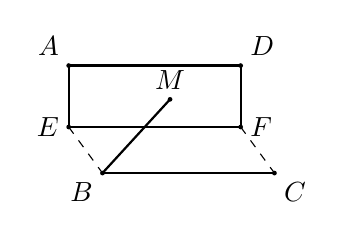
\begin{tikzpicture}[scale=0.78]
  \coordinate (A) at (0,2);
  \coordinate (D) at (2.8,2);
  \coordinate (E) at (0,1);
  \coordinate (F) at (2.8,1);
  \coordinate (B) at (0.55,0.25);
  \coordinate (C) at (3.35,0.25);
  \coordinate (M) at (1.65,1.45);

  \draw[thick] (A)--(D)--(F)--(E)--cycle;
  \draw[thick] (E)--(F);
  \draw[thick] (B)--(C);
  \draw[dashed] (E)--(B) (F)--(C);
  \draw[thick] (B)--(M);

  \fill (A) circle (1.1pt) node[above left] {$A$};
  \fill (D) circle (1.1pt) node[above right] {$D$};
  \fill (E) circle (1.1pt) node[left] {$E$};
  \fill (F) circle (1.1pt) node[right] {$F$};
  \fill (B) circle (1.1pt) node[below left] {$B$};
  \fill (C) circle (1.1pt) node[below right] {$C$};
  \fill (M) circle (1.1pt) node[above] {$M$};
\end{tikzpicture}
\end{center}
\nopagebreak[4]
\Needspace{4\baselineskip}
\textbf{解析}

\Needspace{5\baselineskip}
取折叠后的坐标

\nopagebreak[4]
\[
E=(0,0,0),\quad F=(2,0,0),\quad A=(0,1,0),\quad D=(2,1,0),
\]

\nopagebreak[4]
\[
B=(0,0,-1),\quad C=(2,0,-1),\quad M=(u,v,0).
\]

\Needspace{5\baselineskip}
由 $\angle MBE=\angle MBC$，比较两个余弦值得 $u=1$。直线 $MB$ 的方向向量为 $(1,v,1)$，平面 $BCF$ 为 $y=0$，故

\nopagebreak[4]
\[
\tan\angle(MB,\text{\text{平面} }BCF)=\frac{v}{\sqrt{1^2+1^2}}=\frac v{\sqrt2}.
\]

由题设等于 $1/2$，得 $v=\sqrt2/2$。点到 $EF$ 的距离就是 $v$。

\gkanswer{答案：$\dfrac{\sqrt2}{2}$。}

\end{answer}
\begin{answer}
\gksolhead{16}{}

\textbf{题目}：

\Needspace{5\baselineskip}
对于任意两个复数 $z_1=x_1+y_1i$、$z_2=x_2+y_2i$（$x_1\text{、}y_1\text{、}x_2\text{、}y_2$ 为实数），定义运算 $\odot$ 为

\nopagebreak[4]
\[
z_1\odot z_2=x_1x_2+y_1y_2.
\]

设非零复数 $w_1\text{、}w_2$ 在复平面内对应的点分别为 $P_1\text{、}P_2$，点 $O$ 为坐标原点。如果 $w_1\odot w_2=0$，那么在 $\triangle P_1OP_2$ 中，$\angle P_1OP_2$ 的大小为\gkblank{}。

\Needspace{4\baselineskip}
\textbf{解析}

由 $z_1\odot z_2=x_1x_2+y_1y_2=0$，可知对应向量 $(x_1,y_1)$、$(x_2,y_2)$ 的内积为零。两向量非零，所以夹角为直角。

\gkanswer{答案：$90^\circ$。}

\end{answer}
\gkpart{三、解答题}

\begin{answer}
\gksolhead{17}{}

\textbf{题目}：

\Needspace{5\baselineskip}
在 $\triangle ABC$ 中，已知 $A\text{、}B\text{、}C$ 成等差数列，求

\nopagebreak[4]
\[
\tan\frac A2+\tan\frac C2+\sqrt3\tan\frac A2\tan\frac C2
\]

的值。

\Needspace{4\baselineskip}
\textbf{解析}

\Needspace{5\baselineskip}
$A\text{、}B\text{、}C$ 成等差数列且 $A+B+C=\pi$，故 $B=\pi/3$，从而 $A+C=2\pi/3$。令 $x=\tan(A/2)$、$y=\tan(C/2)$，则

\nopagebreak[4]
\[
\frac{x+y}{1-xy}=\tan\frac{A+C}{2}=\sqrt3.
\]

\Needspace{5\baselineskip}
所以 $x+y=\sqrt3(1-xy)$，所求式为

\nopagebreak[4]
\[
x+y+\sqrt3xy=\sqrt3.
\]

\gkanswer{答案：$\sqrt3$。}

\end{answer}
\begin{answer}
\gksolhead{18}{}

\textbf{题目}：

已知函数 $f(x)$ 是偶函数，而且在 $(0,+\infty)$ 上是增函数，判断 $f(x)$ 在 $(-\infty,0)$ 上是增函数还是减函数，并证明你的判断。

\Needspace{4\baselineskip}
\textbf{解析}

\Needspace{5\baselineskip}
若 $x_1<x_2<0$，则 $-x_1>-x_2>0$。由偶性和正半轴上的增性，

\nopagebreak[4]
\[
f(x_1)=f(-x_1)>f(-x_2)=f(x_2).
\]

故 $f(x)$ 在 $(-\infty,0)$ 上为减函数。

\gkanswer{答案：在 $(-\infty,0)$ 上为减函数。}

\end{answer}
\begin{answer}
\gksolhead{19}{}

\textbf{题目}：

在三棱锥 $S-ABC$ 中，如图，$\angle SAB=\angle SAC=\angle ACB=90^\circ$，$AC=2$，$BC=\sqrt{13}$，$SB=\sqrt{29}$。
\nopagebreak[4]
\begin{center}% 2002 年春季京蒙皖文卷第 19 题：三棱锥空间图形
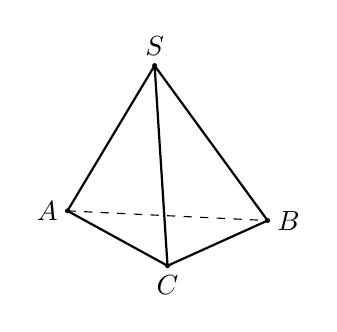
\begin{tikzpicture}[>=stealth, scale=0.82]
  \coordinate (A) at (0,0);
  \coordinate (C) at (1.55,-0.85);
  \coordinate (B) at (3.1,-0.15);
  \coordinate (S) at (1.35,2.25);

  \draw[thick] (A)--(C)--(B);
  \draw[dashed] (A)--(B);
  \draw[thick] (S)--(A) (S)--(B) (S)--(C);

  \fill (A) circle (1.1pt) node[left] {$A$};
  \fill (B) circle (1.1pt) node[right] {$B$};
  \fill (C) circle (1.1pt) node[below] {$C$};
  \fill (S) circle (1.1pt) node[above] {$S$};
\end{tikzpicture}
\end{center}
\nopagebreak[4]
（1） 证明：$SC\perp BC$；

（2） 求侧面 $SBC$ 与底面 $ABC$ 所成的二面角大小；

（3） 求三棱锥的体积 $V_{S-ABC}$。

\Needspace{4\baselineskip}
\textbf{解析}

\Needspace{5\baselineskip}
建立坐标系，取

\nopagebreak[4]
\[
A=(0,0,0),\quad C=(0,2,0),\quad B=(\sqrt{13},2,0),\quad S=(0,0,2\sqrt3).
\]

由 $SB^2=13+4+12=29$，这些坐标满足题设。

\gksubpart{(1)}

\nopagebreak[4]
\[
\overrightarrow{SC}=(0,2,-2\sqrt3),\qquad
\overrightarrow{BC}=(-\sqrt{13},0,0),
\]

两向量内积为零，故 $SC\perp BC$。

\gksubpart{(2)}

\Needspace{5\baselineskip}
平面 $ABC$ 的法向量可取 $(0,0,1)$。平面 $SBC$ 的法向量可取

\nopagebreak[4]
\[
\overrightarrow{CB}\times\overrightarrow{CS}
=(\sqrt{13},0,0)\times(0,-2,2\sqrt3).
\]

两平面所成锐角 $\theta$ 满足 $\cos\theta=1/2$，因此 $\theta=\pi/3$。

\gksubpart{(3)}

\Needspace{5\baselineskip}
底面面积为

\nopagebreak[4]
\[
S_{\triangle ABC}=\frac12\cdot AC\cdot\sqrt{13}=\sqrt{13}.
\]

\Needspace{5\baselineskip}
棱锥高为 $SA=2\sqrt3$，故

\nopagebreak[4]
\[
V_{S-ABC}=\frac13\sqrt{13}\cdot2\sqrt3=\frac{2\sqrt{39}}3.
\]

\nopagebreak[4]
\[
\text{（1） }SC\perp BC;\qquad
\text{（2） }\frac\pi3;\qquad
\text{（3） }\frac{2\sqrt{39}}3.
\]

\gkanswer{答案（1）：见解析。}

\gkanswer{答案（2）：$\dfrac\pi3$。}

\gkanswer{答案（3）：$\dfrac{2\sqrt{39}}3$。}

\end{answer}
\begin{answer}
\gksolhead{20}{}

\textbf{题目}：

假设 A 型进口车关税税率在 2001 年是 100\%，在 2006 年是 25\%，2001 年 A 型进口车每辆价格为 64 万元（其中含 32 万元关税税款）。

（1） 已知与 A 型车性能相近的 B 型国产车，2001 年每辆价格为 46 万元。若 A 型车的价格只受关税降低的影响，为了保证 2006 年 B 型车的价格不高于 A 型车价格的 90\%，B 型车价格要逐年降低，问平均每年至少下降多少万元？

（2） 某人在 2001 年将 33 万元存入银行，假设银行扣利息税后的年利率为 1.8\%（5 年内不变），且每年按复利计算（上一年的利息计入第二年的本金），那么五年到期时这笔钱连本带息是否一定够买按（1）中所述降价后的 B 型车一辆？

\Needspace{4\baselineskip}
\textbf{解析}

\gksubpart{(1)}

\Needspace{5\baselineskip}
A 型车去除关税后的价格为 $32$ 万元，2006 年含税价格为

\nopagebreak[4]
\[
32(1+25\%)=40\text{ \text{万元}}.
\]

\Needspace{5\baselineskip}
B 型车价格上限为 $40\times90\%=36$ 万元。从 46 万元降至不超过 36 万元，5 年平均至少下降

\nopagebreak[4]
\[
\frac{46-36}{5}=2\text{ \text{万元}}.
\]

\gksubpart{(2)}

\Needspace{5\baselineskip}
按每年平均下降 2 万元计算，2006 年 B 型车价格为 36 万元；存款本息为

\nopagebreak[4]
\[
33(1.018)^5\approx36.08\text{ \text{万元}}>36\text{ \text{万元}}.
\]

因此一定够买。

\gkanswer{答案（1）：平均每年至少下降 $2$ 万元。}

\gkanswer{答案（2）：一定够买。}

\end{answer}
\begin{answer}
\gksolhead{21}{}

\textbf{题目}：

已知某椭圆的焦点是 $F_1(-4,0)$、$F_2(4,0)$，过点 $F_2$ 并垂直于 $x$ 轴的直线与椭圆的一个交点为 $B$，且 $|F_1B|+|F_2B|=10$。椭圆上不同的两点 $A(x_1,y_1)$、$C(x_2,y_2)$ 满足条件：$|F_2A|\text{、}|F_2B|\text{、}|F_2C|$ 成等差数列。

（1） 求该椭圆的方程；

（2） 求弦 $AC$ 中点的横坐标。

\Needspace{4\baselineskip}
\textbf{解析}

\gksubpart{(1)}

\Needspace{5\baselineskip}
椭圆焦半距 $c=4$，由 $|F_1B|+|F_2B|=10$ 得 $2a=10$，所以 $a=5$，$b^2=25-16=9$，方程为

\nopagebreak[4]
\[
\frac{x^2}{25}+\frac{y^2}{9}=1.
\]

\gksubpart{(2)}

\Needspace{5\baselineskip}
对椭圆上任意点 $P(x,y)$，右焦点距离满足

\nopagebreak[4]
\[
|F_2P|=a-\frac ca x=5-\frac45x.
\]

\Needspace{5\baselineskip}
已知 $|F_2A|\text{、}|F_2B|\text{、}|F_2C|$ 成等差数列，且 $B=(4,9/5)$，故

\nopagebreak[4]
\[
|F_2A|+|F_2C|=2|F_2B|=\frac{18}{5}.
\]

\Needspace{5\baselineskip}
于是

\nopagebreak[4]
\[
10-\frac45(x_1+x_2)=\frac{18}{5},
\qquad x_1+x_2=8.
\]

弦 $AC$ 中点的横坐标为 $4$。

\gkanswer{答案（1）：$\dfrac{x^2}{25}+\dfrac{y^2}{9}=1$。}

\gkanswer{答案（2）：弦 $AC$ 中点的横坐标为 $4$。}

\end{answer}
\begin{answer}
\gksolhead{22}{}

\textbf{题目}：

已知点的序列 $A_n(x_n,0)$，$n\in\mathbb N$，其中 $x_1=0$，$x_2=a$（$a<0$），$A_3$ 是线段 $A_1A_2$ 的中点，$A_4$ 是线段 $A_2A_3$ 的中点，$\cdots$，$A_n$ 是线段 $A_{n-2}A_{n-1}$ 的中点，$\cdots$。

（1） 写出 $x_n$ 与 $x_{n-1}\text{、}x_{n-2}$ 之间的关系式（$n\ge3$）；

（2） 设 $a_n=x_{n+1}-x_n$，计算 $a_1\text{、}a_2\text{、}a_3$，由此推测数列 $\{a_n\}$ 的通项公式，并加以证明；

（3） 求 $\displaystyle\lim_{n\to\infty}x_n$。

\Needspace{4\baselineskip}
\textbf{解析}

\gksubpart{(1)}

\Needspace{5\baselineskip}
由中点定义，

\nopagebreak[4]
\[
x_n=\frac{x_{n-1}+x_{n-2}}2,\qquad n\ge3.
\]

\gksubpart{(2)}

\Needspace{5\baselineskip}
令 $a_n=x_{n+1}-x_n$，则

\nopagebreak[4]
\[
a_n=\frac{x_n+x_{n-1}}2-x_n=-\frac12a_{n-1}.
\]

\Needspace{5\baselineskip}
由 $a_1=a$ 得

\nopagebreak[4]
\[
a_n=a\left(-\frac12\right)^{n-1}.
\]

\gksubpart{(3)}

\Needspace{5\baselineskip}
因此

\nopagebreak[4]
\[
x_n=x_1+\sum_{j=1}^{n-1}a_j
=a\sum_{j=0}^{n-2}\left(-\frac12\right)^j
=\frac{2a}{3}\left(1-\left(-\frac12\right)^{n-1}\right).
\]

\Needspace{5\baselineskip}
故

\nopagebreak[4]
\[
\lim_{n\to\infty}x_n=\frac{2a}{3}.
\]

\gkanswer{答案（1）：$x_n=\dfrac{x_{n-1}+x_{n-2}}2$。}

\gkanswer{答案（2）：$a_1=a$，$a_2=-\dfrac a2$，$a_3=\dfrac a4$，$a_n=a\left(-\dfrac12\right)^{n-1}$。}

\gkanswer{答案（3）：$\displaystyle\lim_{n\to\infty}x_n=\dfrac{2a}{3}$。}

\end{answer}